\section{The Reward Function}
\label{section:the-reward-function}

Learning in single-step environments mainly requires that the agent has global information about the whole learning task. I.\,e., the optimal representation of an XCS's \emph{reward function} is also the solution of the actual problem. In the 6-multiplexer problem, the reward function already contains the table of the 6-multiplexer itself, which provides a straightforward evaluation of classifiers.

In multi-step environments, the environment will only return a reward value equal to $1$, if the animat reaches the goal position. If not, the reward will be $0$ at all other positions. Since an animat has only access to local information, it is the individual agent's task to compute different reward values for all possible positions in a Maze to differentiate which movement is preferred at each step. In general, this is achieved by \emph{back propagating} the reward of the environment to previous actions. The reward is discounted in order to favor shorter routes. If the animat reaches the goal position, the scenario will be repeated a number of times. In other words, to find the optimal (shortest) route, i.\,e., the global reward function, the agent must be able to distinguish between all positions, i.\,e., the scenario must fulfil the Markov property.

In the predator/prey scenario, the nature of the reward function is not obvious. Since the prey continuously moves, which provides a dynamically changing environment, repetition of the learning process seems not possible. Moreover, the environment does not possess the Markov property, since all agents move, decide, learn in parallel, and previously gathered information does not seem valid any longer. Thus, global information and therefore a global reward function cannot be constructed from the local agent's view. Previous actions require a direct reward process. Additionally, points in time have to be determined, when a reward is distributed on past condition-action-mappings, even if the simulation (i.\,e., the observation task) is continuously performed.

To fulfil these requirements, a new mechanism of reward distribution in such dynamic predator/prey scenarios is proposed. Firstly, an expansion of the reward function by including sensory information is implemented. 
%the \emph{environmental reward function} is chosen by testing static strategies 
(see Section~\ref{subsection:environment-reward-function}). Then, predators will record the resulting reward values of previous actions and will create \emph{events}, if the reward values change or if no change occurs for a specific amount of time (see Section~\ref{subsection:events}). Finally, previously executed actions will be rewarded according to the type of the event and the time difference between the current and the last event (see Section~\ref{subsection:reward-distribution}). We explain this modified multi-step learning in the following.


\subsection{Environmental Reward Function}
\label{subsection:environment-reward-function}

In typical Maze environments, an animat will be rewarded by the environment if it reaches a sparingly distributed goal position. In the context of a predator/prey scenario following a dynamic observation task, the state \emph{reaching the goal position} could be interpreted as \emph{having the prey in the observation range}. Then, the local goal would be equal to the global goal from single-agent's view. Another approach could utilize more complex sensor data on an agent's level instead of being restricted to using a reward function modeled after the global goal (e.g. \emph{goal position is reached} and the \emph{goal position is not reached}). Since the number of possible reward functions, which include more sensor data, seems unlimited and not all functions can be tested in a reasonable amount of time, the investigated approach followed the idea of exploring the search space using static strategies and then testing promising functions on LCSs. In the following a selection of three different strategies are presented. 

%Thus, a collaborative agent behavior, where an agent always tries to contribute to a maximal number of observations, will base on a combination of the two following main strategies: 

\begin{itemize}
	\item {\bf Selfish behavior (observation range)}: Move towards the prey when it is in {\bf observation range}. Otherwise move in a randomly chosen direction.
	\item {\bf Selfish behavior (sight range)}: Move towards the prey when it is in {\bf sight range}. Otherwise move in a randomly chosen direction.
	\item {\bf Cooperative behavior}: Move towards the prey when it is in {\bf sight range}. Otherwise move in a randomly chosen direction without having other agents in the individual {\bf observation range}.
\end{itemize}

Although static strategies do not use a reward function, they still evaluate condition-action-mappings either as \emph{good} (i.\,e., move on that direction) or as \emph{bad} (i.\,e., do not move on that direction), thus an appropriate reward function can be implemented. We define the return value of such a reward function as the \emph{base reward} and the function itself as the \emph{environmental reward function}.

While the implementation of the \emph{selfish behavior} strategy with only one prey on the field is trivial, the \emph{cooperative behavior} strategy requires multiple return values of the reward function. Since a typical XCS implementation \cite{BW02} uses only a binary-coded reward function, an approximation will be used to differentiate between these different system states: The reward function will return $1$, if no other predator is in the personal observation range or if the prey is in the personal sight range (or both will be true), and $0$ otherwise. 

% the following approximation of the reward function $r_{b}(s_{a}, s_{g})$ with $s_{a}, s_{g}$ being indicators whether the goal object is in sight or observation range ($s_{g} = true$) and whether any other agent is in observation range ($s_{a} = true$) is used:
%$$
%r_{b}(s_{a}, s_{g}) = \left\{ \begin{array}{rl}
%  0 & s_{a} \wedge \overline{s_{g}} \\
%  1 & \overline{s_{a}} \vee s_{g}
%       \end{array} \right.
%$$

% As further adaptions to the reward is necessary the value this function returns will be called ``base reward'' and the function itself ``environmental reward function''. In the following section the actual reward for the rules of the XCS will be calculated. 

\subsection{Events}
\label{subsection:events}

In the usual implementation of an XCS~\cite{BW02} any positive \emph{base reward} is distributed whenever an animat reaches a goal position and the scenario is then restarted. Here, we analyze past \emph{base reward} values and generate so called \emph{events} when either the \emph{base reward} value has changed or when no change occurs for a certain period of time.

Assuming that a predator has taken a good decision when the prey comes into the sight range of predator (or the predator leaves the sight ranges of all other predators) we define such a situation change as a \emph{positive event}. Moreover, loosing the prey or coming into the sight ranges of other predators will be called a \emph{negative event}. In other words, a positive event always occurs whenever the \emph{base reward} changes from $0$ to $1$, a negative event occurs whenever the \emph{base reward} changes from $1$ to $0$, as depicted in Figure~\ref{figure:positive-negative-events}.

\begin{figure*}[ht]
  \subfigure[Example of a series of \emph{base rewards}, which lead to both \emph{positive} and \emph{negative events}.]{
  	\label{figure:positive-negative-events}
  	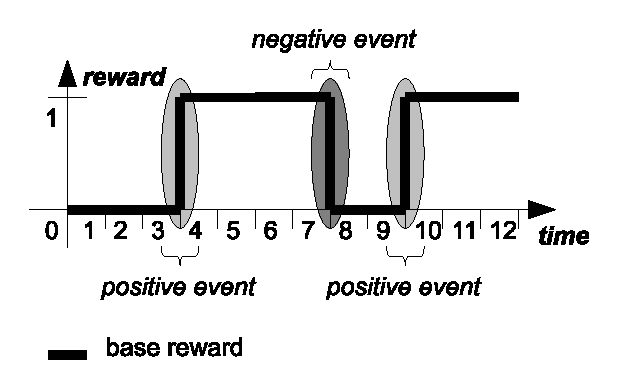
\includegraphics[width=0.32\textwidth]{positive_negative_events.eps}}\hfill
  \subfigure[Example of a series of \emph{base rewards}, which force a \emph{neutral event} (\emph{maxStackSize} = 8).]{
  	\label{figure:neutral-event}
  	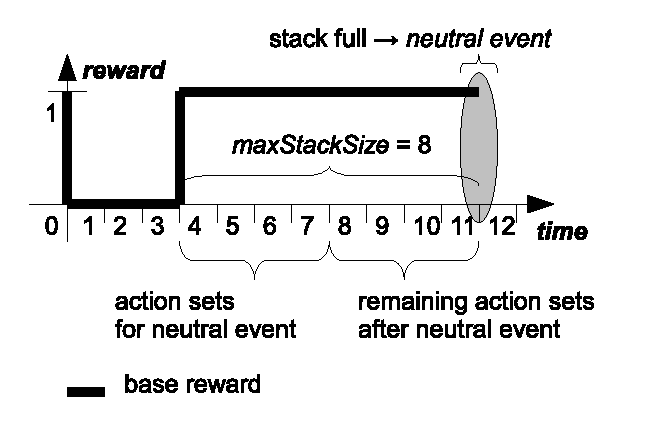
\includegraphics[width=0.32\textwidth]{neutral_event.eps}}\hfill
  \subfigure[Reward distribution mechanism for a number of positive and negative events]{
  	\label{figure:saved-rewards}
  	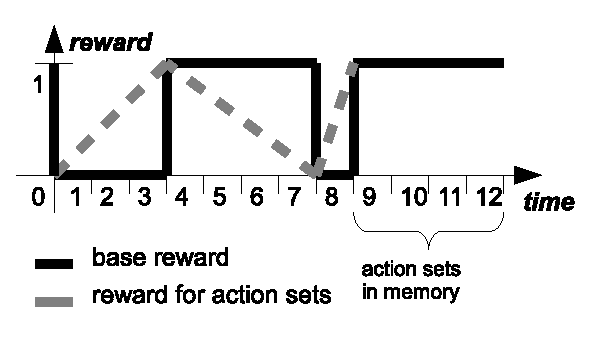
\includegraphics[width=0.32\textwidth]{saved_rewards.eps}}
	\caption{\mathversion{bold}Calculation of the reward of individual action sets by analyzing the \emph{base reward}}
	\label{figure:experiment}
\end{figure*}

%\begin{figure}[ht]
%\centerline{	
%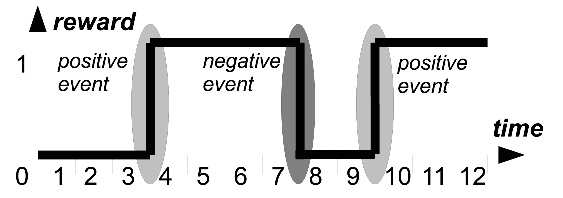
\includegraphics[scale=0.75]{positive_negative_events}
%}
%\caption{Example of a series of base rewards that lead to positive and negative events.}
%\label{figure:positive-negative-events}
%\end{figure}

Nevertheless, a predator will also contribute to a collaborative group behavior, if the prey is never seen in the personal observation range and other predators are also stayed away. Hence, a predator will never encounter an event and no reward will be computed to evaluate past actions. Thus, the number of learning cycles -- that can occur without encountering an event -- have been limited by a variable \emph{maxStackSize}. If this step counter reaches the predefined threshold, a \emph{neutral event} will occur (see Figure~\ref{figure:neutral-event}). Then, the step counter is reset to $0$ and the LCS waits for a new event or the step counter again passes the threshold of the \emph{maxStackSize}. Additionally, half of the action sets in the stack are rewarded according to the actual \emph{base reward} value and then discarded.

%\begin{figure}[ht]
%\centerline{	
%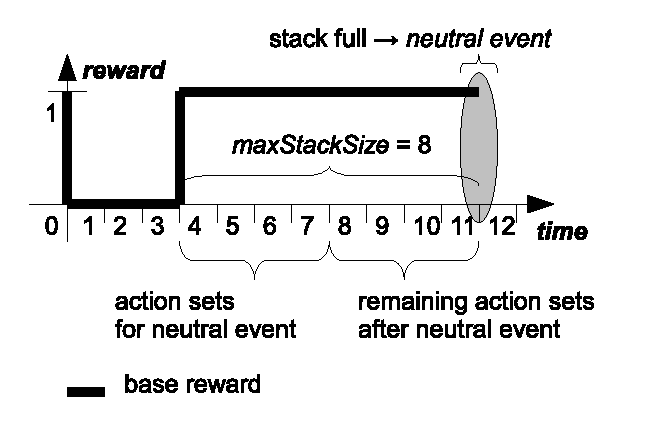
\includegraphics[scale=0.75]{neutral_event}
%}
%\caption{Example of a series of base rewards that lead to neutral event (with %\emph{maxStackSize} = 8).}
%\label{figure:neutral-event}
%\end{figure}

\subsection{Reward Distribution}
\label{subsection:reward-distribution}

The standard implementation of an XCS is based on the assumption that it learns within a MDP. This is expressed in the way the reward is distributed on the classifiers that have contributed to reach the goal. Generally, several repetitions are required to correctly distribute the reward to all classifiers that have contributed to the solution.

In a dynamic scenario, such repetitions are not possible. The scenario is not restarted and the observation task is continuously performed. Thus, a separate mechanism is introduced to reward previous (contributing) actions as well. This new approach stores not only the last, but all previous actions. We admit that such a memory mechanism does not necessarily restore the Markov property (the scenario is obviously a NOMDP, as explained in Section~\ref{subsection:scenario-classification}). However, it directly associates a changing base reward value with previous steps, which have contributed to the success (or to a failure), since the last change of the \emph{base reward} has been observed. % and an improvement in the performance is to be expected.
Thus, when (and only when) an event occurs, the reward will be distributed among the entries of the action sets that have been stored, since the last event has been occurred. Moreover, recent actions have probably contributed more to a positive (negative) event than older actions. Hence, they are evaluated with a higher (lower) reward than those actions that were executed several steps before. To realize this \emph{reward distribution} mechanism, a quadratic function is used, which extends the rewarding procedure of the original XCS implementation with $r(a)$ being the \emph{reward} for the \emph{action set} with an age of $a$:
$$ % \begin{equation}
	r(a) = 
	\left\{ \begin{array}{r@{,\quad}l}
		\emph{base reward} & \mbox{\emph{neutral event}}\\  	
		\frac{{a}^{2}}{{\mathrm{size(\emph{action set})}}^{2}} & \mbox{\emph{positive event}} \\
  		\frac{{(1 - a)}^{2}}{{\mathrm{size(\emph{action set})}}^{2}} & \mbox{\emph{negative event}}
  	\end{array} \right.
$$ % \end{equation}

In Figure~\ref{figure:saved-rewards}, an example illustrates this reward distribution mechanism. For simplicity a linear distribution of the reward on previous action sets is displayed, but more sophisticated approaches seems possible. However, significant differences between a linear or a no-linear distribution could not be investigated so far. 

%\begin{figure}[ht]
%\centerline{	
%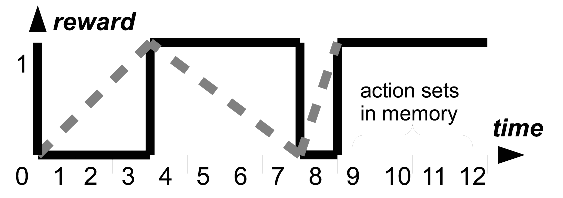
\includegraphics[scale=0.75]{saved_rewards}
%}
%\caption{Schematic presentation of the reward distribution to the action sets over time after several positive and negative events}
%\label{figure:saved-rewards}
%\end{figure}
